All numerical claims are deterministic point estimates from a single fixed Dryden seed~42 (\cref{rem:reproducibility}).

\subsection{Simulation Environment and Campaign Structure}
\label{sec:campaign}


All simulations run in Drake~\cite{drake} with an RK3 continuous-time integrator at a max step of \SI{1}{\milli\second}. Drones and payload are rigid multibody systems; ropes are bead-chain Kelvin--Voigt spring-dampers whose lumped stiffness is justified by \cref{thm:reduction}. Wind is body-frame aerodynamic drag per drone and on the payload, using a Dryden low-altitude turbulence model. \Cref{tab:sim-params} lists the simulator and plant parameters.

\begin{table}[htbp]
  \caption{Simulator and Plant Parameters}
  \label{tab:sim-params}
  \centering
  \begin{tabular}{lrl}
    \toprule
    Parameter                        & Value     & Unit                       \\
    \midrule
    Number of drones $N$             & 5         & ---                        \\
    Drone mass $m_i$                 & 1.5       & \si{\kilo\gram}            \\
    Payload mass $m_L$               & 10        & \si{\kilo\gram}            \\
    Rope rest length $\ell_0$        & 1.25      & \si{\metre}                \\
    Rope stiffness $k$               & 25\,000   & \si{\newton\per\metre}     \\
    Formation ring radius            & 0.80      & \si{\metre}                \\
    Reference trajectory             & 3-D lemniscate & ---               \\
    \quad Horizontal amplitude       & 3.0       & \si{\metre}                \\
    \quad Period (nominal)           & 12        & \si{\second}               \\
    \quad Vertical amplitude         & 0.35      & \si{\metre}                \\
    Wind model                       & Dryden low-altitude & ---          \\
    \quad Mean speed (along $+x$)    & 4         & \si{\metre\per\second}     \\
    \quad $\sigma_u,\;\sigma_v$      & 0.8       & \si{\metre\per\second}     \\
    \quad $\sigma_w$                 & 0.4       & \si{\metre\per\second}     \\
    Turbulence seed                  & 42        & ---                        \\
    Simulation duration              & 30        & \si{\second}               \\
    Pre-fault cruise window          & $[8,\,12]$  & \si{\second}             \\
    Actuator thrust ceiling          & 150       & \si{\newton}               \\
    MPC tension ceiling (V6 only)    & 100       & \si{\newton}               \\
    \bottomrule
  \end{tabular}
\end{table}

The campaign structure (\cref{tab:campaign-matrix}) comprises V1--V6 as the pre-declared capability sequence, each adding one stressor, and P2-A--P2-D as targeted ablations. Faults are instantaneous: the rope tension is set to zero; survivors continue without notification.

\begin{table*}[htbp]
  \caption{Simulation campaign matrix. Capability-demonstration variants V1--V6 and targeted ablations P2-A through P2-D.}
  \label{tab:campaign-matrix}
  \centering
  \begin{tabular}{llp{5.5cm}cp{5cm}}
    \toprule
    Tag & Controller            & Fault Schedule                                                                          & Wind & Purpose \\
    \midrule
    \multicolumn{5}{l}{\textit{Capability Demonstration (C1--C3 primary evidence)}} \\[\smallskipamount]
    V1 & Baseline QP           & None                                                                                    & No   & Nominal tracking floor; C2 bound check \\
    V2 & Baseline QP           & None                                                                                    & Yes  & Wind-rejection baseline \\
    V3 & Baseline QP           & Drone~0 at $t{=}\SI{12}{s}$                                                             & Yes  & Single-fault recovery \\
    V4 & Baseline QP           & Drone~0 at $t{=}\SI{12}{s}$; Drone~2 at $t{=}\SI{17}{s}$ \mbox{($\Delta t{=}\SI{5}{s}$)}  & Yes  & Dual fault; dwell margin \SI{2.76}{s} \\
    V5 & Baseline QP           & Drone~0 at $t{=}\SI{12}{s}$; Drone~2 at $t{=}\SI{22}{s}$ \mbox{($\Delta t{=}\SI{10}{s}$)} & Yes  & Dual fault; dwell margin \SI{7.76}{s} \\
    V6 & Full stack            & Same as V4                                                                              & Yes  & Full-stack integration; hardest scenario \\
       & (MPC$+L_1+$reshape)  &                                                                                         &      & \\
    \midrule
    \multicolumn{5}{l}{\textit{Targeted Ablations (causal isolation and domain characterization)}} \\[\smallskipamount]
    P2-A & Baseline, FF disabled & V3, V4, V5 schedules                                                                 & Yes  & Feed-forward causality (C2) \\
    P2-B & Baseline / $+L_1$    & None                                                                                  & No   & Mass-mismatch robustness (C3-$L_1$) \\
    P2-C & MPC, ceiling sweep   & V4 schedule                                                                           & Yes  & Tension-ceiling sensitivity (C3-MPC) \\
    P2-D & Baseline + reshape   & V4 schedule, period $T_{\mathrm{ref}} \in \{8,10,12\}$~s                              & Yes  & Reshape benefit vs.\ trajectory period (C3-Reshape) \\
    \bottomrule
  \end{tabular}
\end{table*}

\paragraph{Admissibility-domain audit (H1 and H3).} \Cref{thm:reduction} and \cref{thm:hybrid-stability} require three gates to hold on the demonstrated trajectory: H1a (no slack run $> \SI{40}{\milli\second}$), H1b (aggregate slack duty cycle $\le 2.5\%$), and H3 (QP active-set transition fraction $\le 1\%$). \Cref{tab:domain-audit} reports measurements for V1--V6: every variant passes with margin. Worst observed values are \SI{35.8}{\milli\second} (H1a; V2--V5, $\SI{4.2}{\milli\second}$ margin), $1.66\%$ (H1b; V6, $0.84$~pp margin), and $0.10\%$ (H3; V4--V6, $0.90$~pp margin). These measurements certify domain membership for the demonstrated mission family but do not prove H1--H3 for all references, wind, or fault schedules; the audit must be repeated for new missions. V6's lower H1a ($\SI{31.4}{\milli\second}$) is consistent with MPC damping high-frequency QP transitions.

\begin{table}[htbp]
  \caption{Domain gate audit. Thresholds: H1a $\le \SI{40}{\milli\second}$; H1b $\le 2.5\,\%$; H3 $\le 1.0\,\%$.}
  \label{tab:domain-audit}
  \centering
  \small
  \renewcommand{\arraystretch}{1.05}
  \begin{tabular}{lcccccc}
    \toprule
    & \multicolumn{2}{c}{H1a (ms)} & \multicolumn{2}{c}{H1b (\%)} & \multicolumn{2}{c}{H3 (\%)} \\
    \cmidrule(lr){2-3}\cmidrule(lr){4-5}\cmidrule(lr){6-7}
    Variant & Value & Pass & Value & Pass & Value & Pass \\
    \midrule
    V1 & 21.2 & \checkmark & 1.34 & \checkmark & 0.07 & \checkmark \\
    V2 & 35.8 & \checkmark & 1.52 & \checkmark & 0.07 & \checkmark \\
    V3 & 35.8 & \checkmark & 1.52 & \checkmark & 0.09 & \checkmark \\
    V4 & 35.8 & \checkmark & 1.52 & \checkmark & 0.10 & \checkmark \\
    V5 & 35.8 & \checkmark & 1.52 & \checkmark & 0.10 & \checkmark \\
    V6 & 31.4 & \checkmark & 1.66 & \checkmark & 0.10 & \checkmark \\
    \midrule
    Gate & \multicolumn{2}{c}{$\le 40$} & \multicolumn{2}{c}{$\le 2.5$} & \multicolumn{2}{c}{$\le 1.0$} \\
    \bottomrule
  \end{tabular}
\end{table}

\paragraph{Statistical scope.} All campaigns use fixed Dryden seed~42 (reproducible $2\sigma$ exceedance within $[8,12]\,\si{\second}$); reported RMSE, sag, and ablation values are deterministic point estimates. CRN-paired replication with bootstrap CIs is follow-up work.

\paragraph{Scope.} V1--V6 begin slightly slack ($\SI{1.17}{\metre}$ vs.\ $\SI{1.25}{\metre}$ rest length); pickup engages within the first tick and the evaluation window $[8,30]\,\si{\second}$ excludes the transient.

\subsection{Reduction-Fidelity Audit}
\label{sec:VI-reduction}


Three quantities must be kept distinct:
\begin{itemize}[leftmargin=1.5em,noitemsep]
  \item $T_i^{\mathrm{qs}} \triangleq k_{\mathrm{eff}}(\ell_i - L)^+$ --- the \emph{per-rope quasi-static} tension (same $\ell_i$ as the physical rope); \cref{thm:reduction} bounds $|T_i^{\mathrm{KV}} - T_i^{\mathrm{qs}}|$ at $\le C_1\delta + C_2\eta_{\max} \approx \SI{0.076}{\newton}$;
  \item $\varepsilon_i \triangleq T_i^{\mathrm{KV}} - T_{\mathrm{eff}}$ --- the \emph{inter-rope asymmetry} around the surviving-rope mean; this is a formation-geometry effect, driven by post-fault load redistribution, and is \emph{not} bounded by \cref{thm:reduction};
  \item trajectory deviation --- the quantity controlled by \cref{thm:hybrid-stability}, which absorbs both $T_i^{\mathrm{qs}}$ and the feed-forward identity.
\end{itemize}

The empirical audit measures $\varepsilon_i = T_i^{\mathrm{KV}} - T_{\mathrm{eff}}$, which is formation-geometry driven and structurally larger than the shape-mode deviation; its role is to characterize post-fault load asymmetry, not to verify the theorem bound.

The domain-gate layer (\cref{tab:domain-audit}) certifies that $\eta$, max slack-run, and QP transition fraction satisfy the theorem hypotheses with margin across all variants; this is the primary certificate.

The \emph{inter-rope dispersion} layer provides additional context. On $[8,30]\,\si{\second}$ for each variant we compute $T_{\mathrm{eff}}(t) = |\mathcal{S}(t)|^{-1} \sum_{i\in\mathcal{S}(t)} T_i^{\mathrm{KV}}(t)$ and $\varepsilon_i(t) = T_i^{\mathrm{KV}}(t) - T_{\mathrm{eff}}(t)$. \Cref{tab:reduction-residuals} reports RMS, P95, and peak of $|\varepsilon_i|$; \cref{fig:reduction-overlay-V4} overlays per-rope $T_i^{\mathrm{KV}}$ against $T_{\mathrm{eff}}$ for V4. The inter-rope asymmetry sits at RMS $\sim\SI{12}{\newton}$ on dual-fault variants ($\approx 60\%$ of nominal per-rope tension), with peaks at $\SI{60}{\newton}$ at the most centripetally-loaded instants. This large dispersion is architecturally expected: after a fault, each surviving rope carries more load and formation angles differ, causing $T_i^{\mathrm{qs}}$ to vary across ropes by the same $O(10)$\,N. It does not contradict the theorem, which bounds $|T_i^{\mathrm{KV}} - T_i^{\mathrm{qs}}|$ at $\approx\SI{0.076}{\newton}$ --- the shape-mode deviation of each rope \emph{from its own} quasi-static baseline. The identity $T_i^{\mathrm{ff}} = T_i$ ensures each drone receives the full asymmetric signal, so the stability analysis need not model the asymmetry analytically (\cref{lem:tension-cancel}). A trajectory-level audit against a reduced-rope simulator is follow-up work.

\begin{table}[htbp]
  \caption{Inter-rope tension asymmetry $|\varepsilon_i| = |T_i^{\mathrm{KV}} - T_{\mathrm{eff}}|$ over $[8,\,30]\,\si{\second}$ cruise, surviving ropes. $T_{\mathrm{eff}}$ is the mean across surviving ropes; this measures formation-geometry load dispersion, \emph{not} the shape-mode deviation bounded by \cref{thm:reduction}. Nominal per-rope tension $m_L g / 5 \approx \SI{19.6}{\newton}$.}
  \label{tab:reduction-residuals}
  \centering
  \small
  \renewcommand{\arraystretch}{1.05}
  \begin{tabular}{lrrr}
    \toprule
    Variant & RMS (N) & P95 (N) & Peak (N) \\
    \midrule
    V1 & 7.4  & 15.5 & 60.5 \\
    V2 & 7.1  & 14.8 & 52.6 \\
    V3 & 12.8 & 22.1 & 52.6 \\
    V4 & 12.4 & 22.5 & 52.6 \\
    V5 & 12.3 & 21.9 & 52.6 \\
    V6 & 12.8 & 23.6 & 60.2 \\
    \bottomrule
  \end{tabular}
\end{table}

\begin{figure}[htbp]
  \centering
  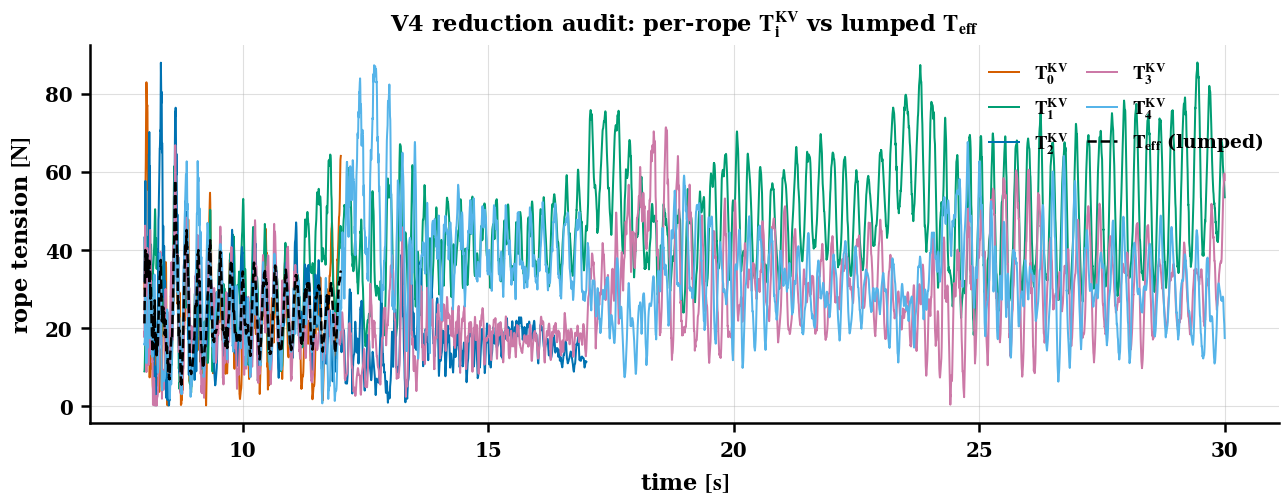
\includegraphics[width=\columnwidth]{Figures/fig_reduction_overlay_V4.png}
  \caption{V4 reduction audit. Coloured: per-rope Kelvin--Voigt truth tension $T_i^{\mathrm{KV}}(t)$ (severed ropes drop to zero at fault). Dashed black: surviving-rope mean $T_{\mathrm{eff}}(t)$. The spread around $T_{\mathrm{eff}}$ is the inter-rope tension asymmetry $\varepsilon_i$ (formation-geometry effect); the shape-mode deviation $|T_i^{\mathrm{KV}} - T_i^{\mathrm{qs}}|$ bounded by \cref{thm:reduction} at $\approx\SI{0.076}{\newton}$ is not visible at this scale.}
  \label{fig:reduction-overlay-V4}
\end{figure}

% ----------------------------------------------------------------
\subsection{Nominal Tracking Performance}
\label{sec:VI-B}
% ----------------------------------------------------------------

V1 (no wind) yields 3-D RMSE $\SI{0.312}{\metre}$ over $[8,30]$~s. The bound of \cref{cor:steady-state} is horizontal-only; V1 horizontal RMSE $\SI{0.306}{\metre}$ matches the predicted $\SI{0.27}{\metre}$ to leading order, with the gap from centripetal acceleration on the curved segments. The 3-D value exceeds the corollary because it accumulates altitude error over the $\pm\SI{0.35}{\metre}$ vertical excursion, which the horizontal-only derivation excludes.

V2 (Dryden wind, $\SI{4}{\metre\per\second}$ mean, seed~42) yields RMSE $\SI{0.312}{\metre}$, indistinguishable from V1 at single-seed precision. The PD/QP layer absorbs the turbulence without adaptive augmentation, exercising the wind margin of \cref{cor:robustness}. \Cref{tab:performance-ci} consolidates per-variant RMSE, sag, and tension; \cref{fig:trajectory-3d-V4} shows the V4 payload trajectory in 3-D with the lemniscate reference, fault events, and three formation snapshots.

\begin{figure*}[htbp]
  \centering
  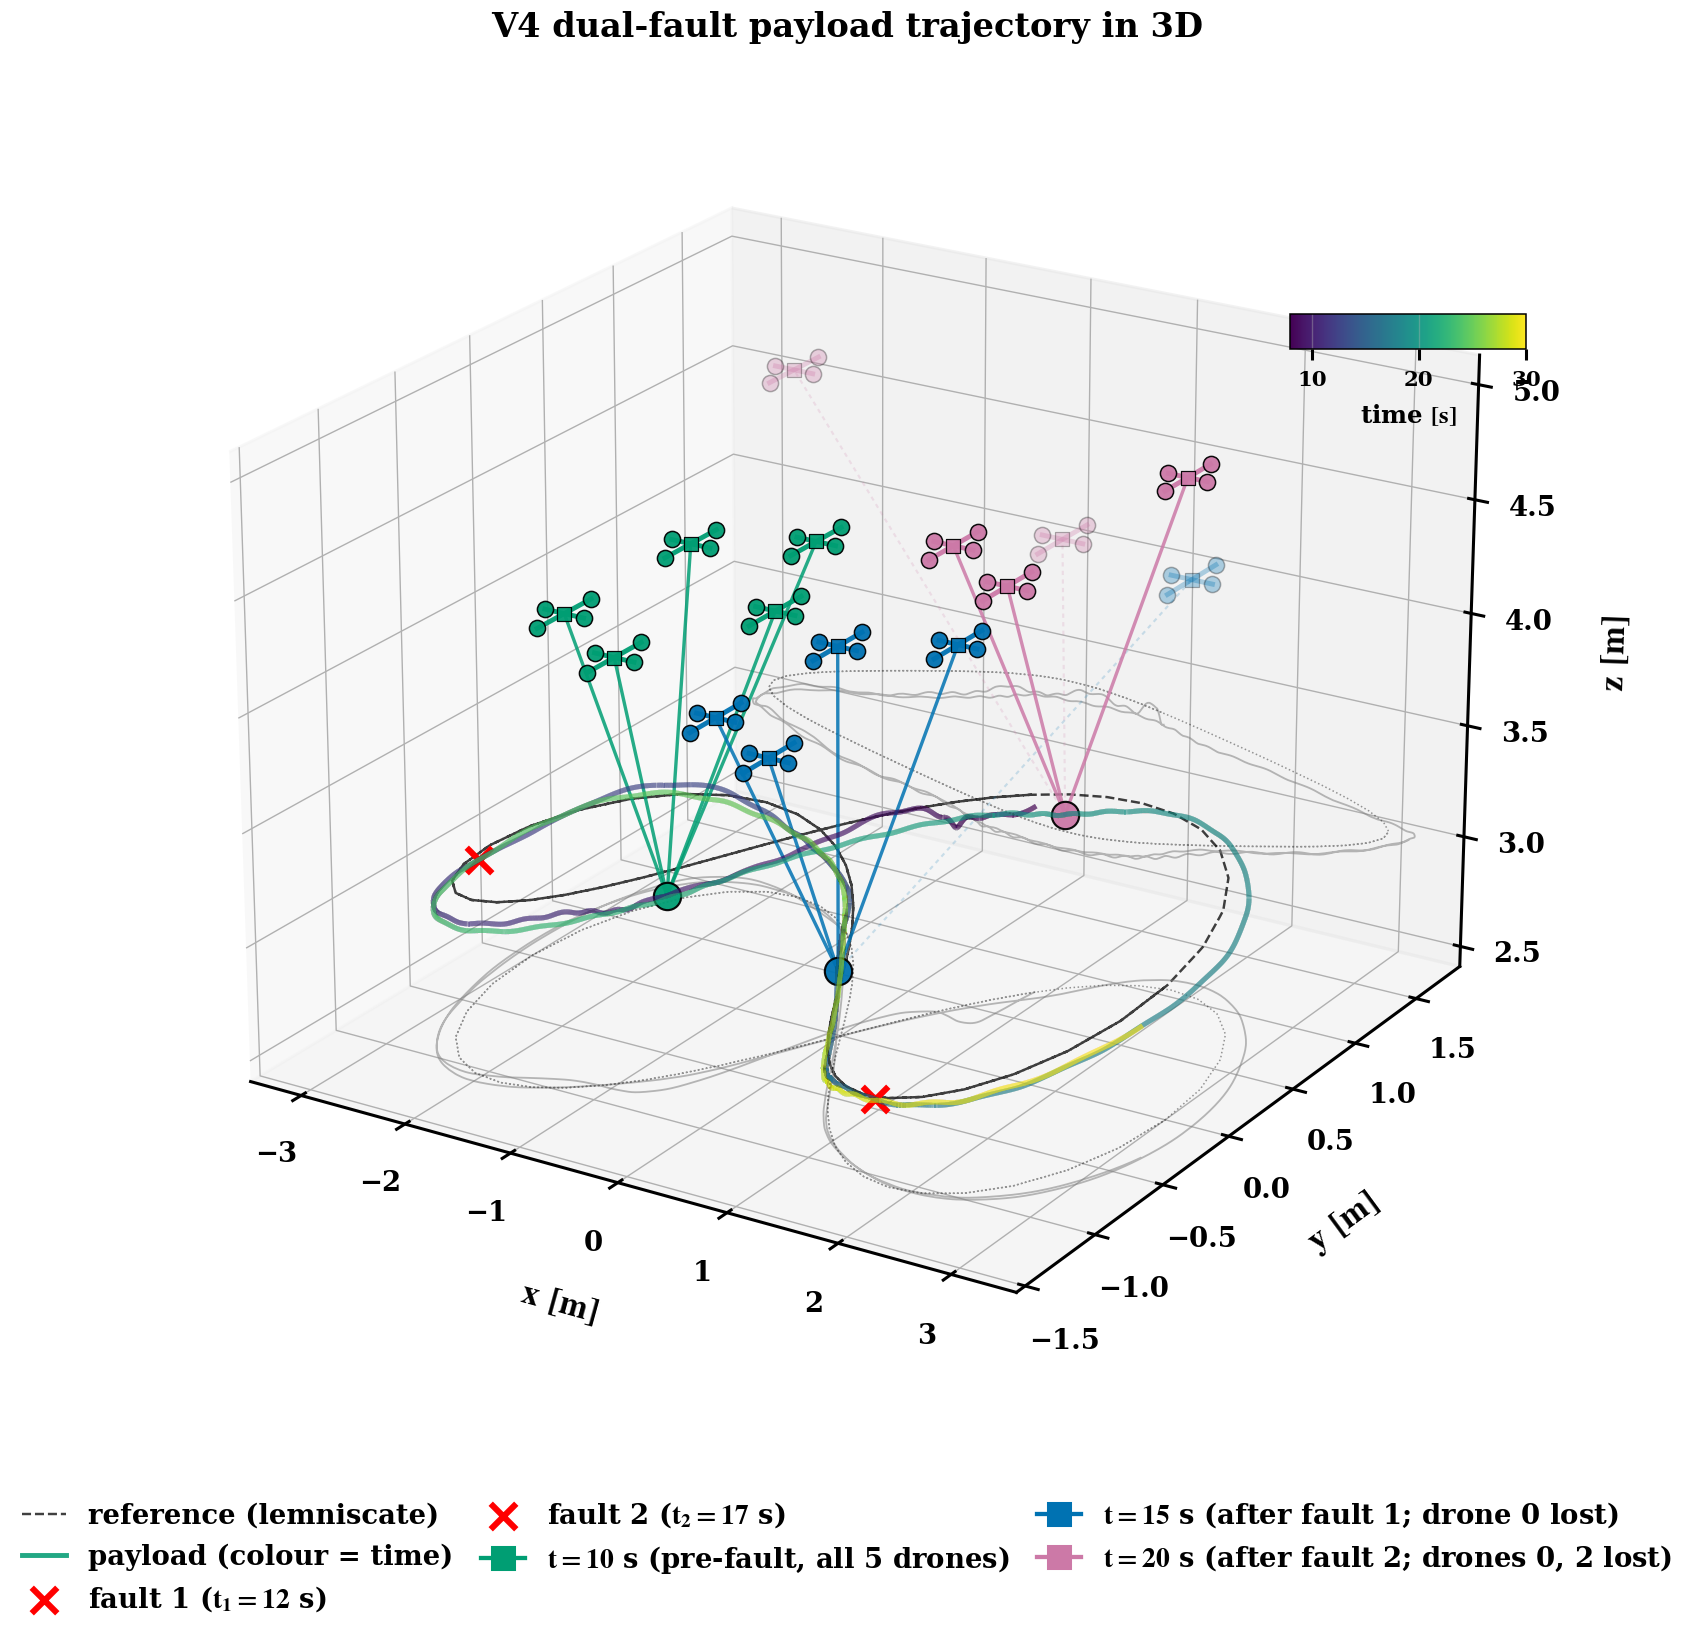
\includegraphics[width=0.92\textwidth]{Figures/fig_trajectory_3d_V4.png}
  \caption{V4 dual-fault payload trajectory. Time-coloured curve: payload over $t \in [8,30]\,\si{\second}$. Dashed: lemniscate reference. Red crosses: fault events at $t_1{=}12$\,s (drone~0) and $t_2{=}17$\,s (drone~2). Formation snapshots at $t\in\{10,15,20\}$\,s show pre-fault, post-fault~1, and post-fault~2 geometries (solid: taut, dashed: severed). Grey shadows: top-down and side-view projections.}
  \label{fig:trajectory-3d-V4}
\end{figure*}

\Cref{tab:performance-ci} reports integrated system-level performance for V1--V6 (deterministic seed-42 estimates). The rightmost column marks each variant against the pre-registered thresholds: 3-D RMSE $\le \SI{0.35}{\metre}$, sag $\le \SI{100}{\milli\metre}$, tension $\le \SI{120}{\newton}$.

\begin{table}[htbp]
  \caption{Integrated system-level performance (V1--V6, seed-42). Acceptance thresholds: RMSE $\le \SI{0.35}{\metre}$; sag $\le \SI{100}{\milli\metre}$; tension $\le \SI{120}{\newton}$.}
  \label{tab:performance-ci}
  \centering
  \small
  \renewcommand{\arraystretch}{1.05}
  \begin{tabular}{lcccc}
    \toprule
    Variant & RMSE & Sag\textsuperscript{peak}
            & Tension\textsuperscript{peak} & Acceptance \\
    \midrule
    V1 & 0.312m & ---  & 105.3N & Pass \\
    V2 & 0.312m & ---  & 104.6N & Pass \\
    V3 & 0.324m & 86.8mm & 104.6N & Pass \\
    V4 & 0.328m & 95.2mm & 104.6N & Pass \\
    V5 & 0.324m & 90.4mm & 104.6N & Pass \\
    V6 & 0.326m & 76.1mm & 107.6N & Pass \\
    \bottomrule
  \end{tabular}
\end{table}

% ----------------------------------------------------------------
\subsection{Fault Progression, Recovery, and Lyapunov Evidence}
\label{sec:VI-C}
% ----------------------------------------------------------------

We audit \cref{thm:hybrid-stability} against three scenarios of increasing severity: V3 (single fault), V4 (dual, $\Delta t = \SI{5}{\second}$), V5 (dual, $\Delta t = \SI{10}{\second}$).

\paragraph{V3 --- single fault.} Drone~0 severs at $t = \SI{12}{\second}$; four survivors respond without fault signals or peer communication. Peak 3-D error $\SI{0.337}{\metre}$, IAE $\SI{0.452}{\metre\second}$, max sag $\SI{85.1}{\milli\metre}$. Settle time is below the \SI{1}{\milli\second} tick resolution (logged as 0~s): the bounded jump of \cref{lem:jump-continuity} at the near-equal-sharing hover point falls below one tick.

\paragraph{V4 --- dual fault, $\Delta t = \SI{5}{\second}$.} Drone~2 severs at $t = \SI{17}{\second}$, $\SI{5}{\second}$ after the first. Peak error $\SI{0.446}{\metre}$, IAE $\SI{0.666}{\metre\second}$, max sag $\SI{79.1}{\milli\metre}$, settle time $\SI{0.158}{\second}$. The second-fault transient decays within the same envelope, consistent with $\rho < 1$.

\paragraph{V5 --- dual fault, $\Delta t = \SI{10}{\second}$.} Extending the gap to $\SI{10}{\second}$ lets the system fully re-settle. The second fault's IAE is $\SI{0.741}{\metre\second}$ ($+11\%$ over V4) reflecting higher cruise speed at $t = \SI{22}{\second}$, not degraded recovery. Max sag $\SI{87.4}{\milli\metre}$; sub-tick settle.

\paragraph{V6 --- full stack.} With MPC~$+L_1$+reshape active, first-fault sag is $\SI{69.9}{\milli\metre}$ ($-12\%$ vs V4), consistent with the stack preserving the envelope while delivering incremental benefit.

\Cref{fig:fault-zoom} shows the fault-centered timeline for V4 with FF-on (solid) vs FF-off (dashed) on the same wind seed: (a)~tracking-error norm, (b)~altitude error exposing the sag differential, (c)~Lyapunov proxy $V(t) = \xi^\top P_v \xi$, allowing direct visual inspection of the bounded jump (\cref{lem:jump-continuity}) and the inter-event contraction (\cref{lem:dwell-decay}) alongside the causal mechanism. V3, V5, FF-held-constant, and per-drone thrust traces are in the supplementary package. Empirical fits on V4 and V5 give peak jump $\hat\chi_{\max} = 1.1\!\times\!10^{-4}$ (V4), $1.3\!\times\!10^{-5}$ (V5)---in units of the dimensionless proxy $V$, not physical units---and dwell-cycle contraction $\hat\rho_{\text{V4}}=0.20$, $\hat\rho_{\text{V5}}=0.045$, both well below the $\rho < 1$ sufficiency bound (\cref{tab:stability-evidence}).

\begin{figure}[htbp]
  \centering
  \subfloat[Tracking-error norm (V4).]{%
    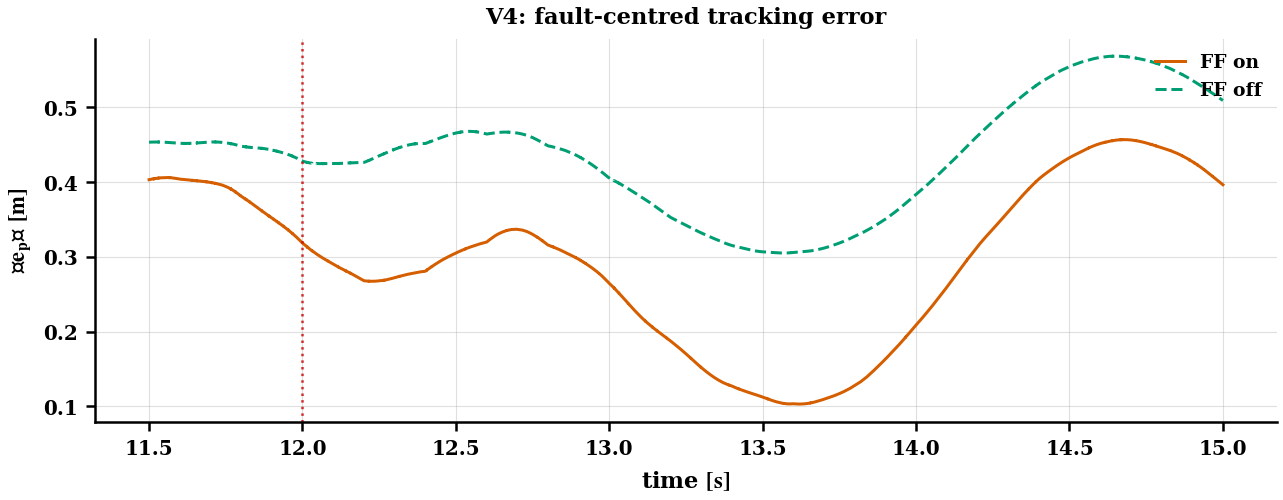
\includegraphics[width=0.95\columnwidth]{Figures/fig_faultzoom_trackerr_V4.png}%
    \label{fig:fz-trackerr-v4}}\hfill
  \subfloat[Payload altitude error (V4).]{%
    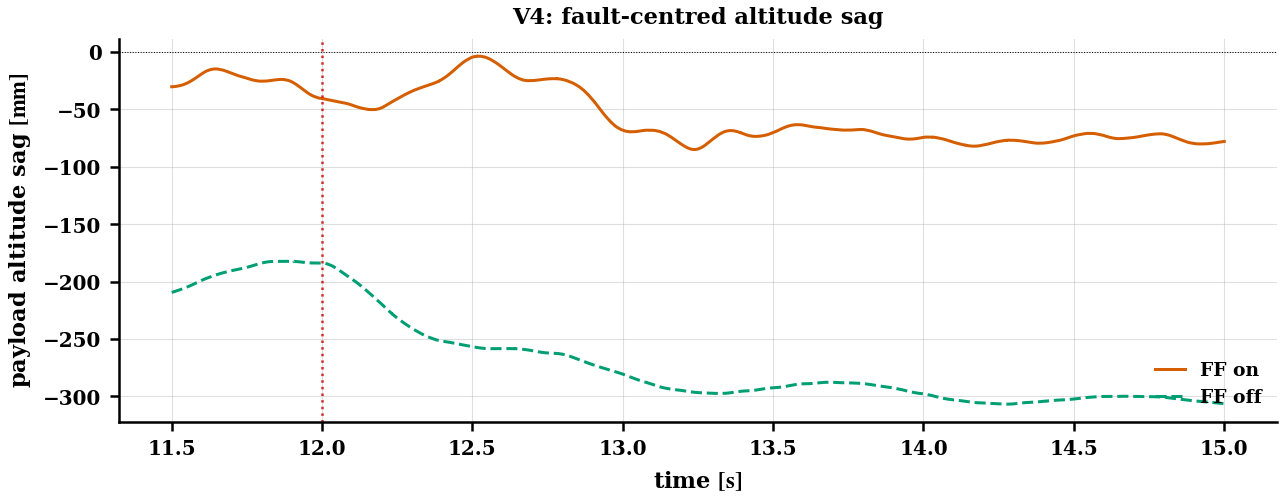
\includegraphics[width=0.95\columnwidth]{Figures/fig_faultzoom_altitude_V4.png}%
    \label{fig:fz-altitude-v4}}\hfill
  \subfloat[Lyapunov proxy $V=\xi^\top P_v\xi$ (V4).]{%
    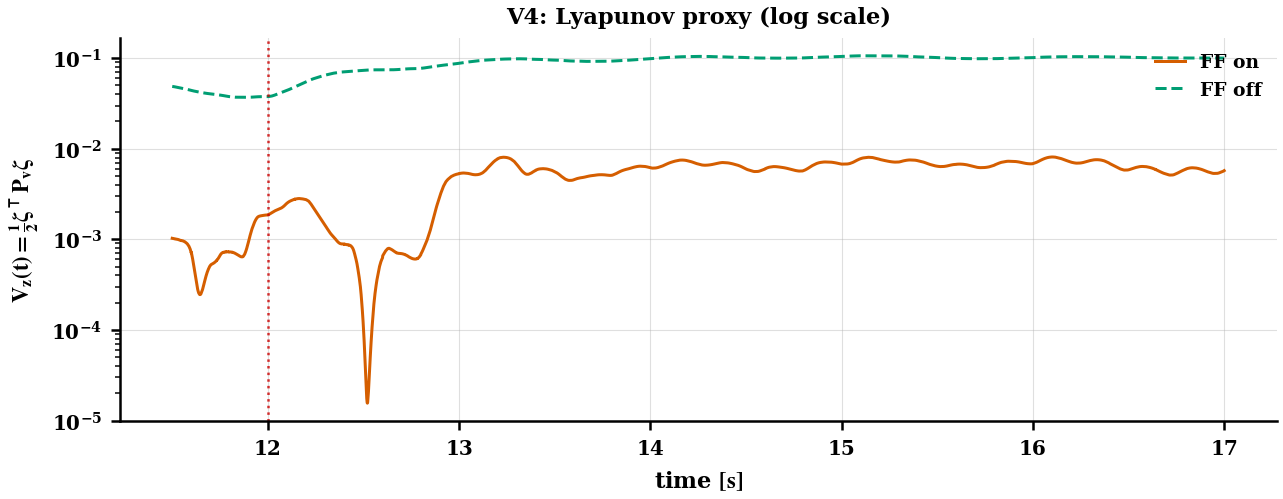
\includegraphics[width=0.95\columnwidth]{Figures/fig_faultzoom_lyapunov_V4.png}%
    \label{fig:fz-lyapunov-v4}}
  \caption{Fault-centered causal ablation on V4, FF-on (solid) vs FF-off (dashed, P2-A) at seed~42. \textit{(a)}~tracking-error norm; \textit{(b)}~altitude error; \textit{(c)}~Lyapunov proxy $V(t)=\xi^\top P_v\xi$, exhibiting the bounded jump of Lemma~\ref{lem:jump-continuity} and the inter-event contraction of Lemma~\ref{lem:dwell-decay}.}
  \label{fig:fault-zoom}
\end{figure}

\subsection{Tension Feedforward Ablation}
\label{sec:VI-D}

The P2-A campaign provides the strongest quantitative evidence for \eqref{eq:Tff} as the causal recovery mechanism. We disable $T_i^{\mathrm{ff}} = T_i$ in the QP layer and repeat V3, V4, V5.

Without the identity, the altitude channel carries an unrejected load increment, inflating both steady-state floor and post-fault Lyapunov jumps (\cref{lem:jump-continuity}); \cref{tab:ff-ablation,fig:fault-zoom} summarize the $34$--$39\%$ RMSE increase and $3.6$--$4.0\times$ peak-sag inflation.

\begin{table}[htbp]
  \caption{Tension feed-forward ablation (P2-A). Cruise-window RMSE (m) and peak post-fault altitude sag (mm) with FF enabled and disabled, per fault schedule.}
  \label{tab:ff-ablation}
  \centering
  \small
  \renewcommand{\arraystretch}{1.05}
  \begin{tabular}{lcccccc}
    \toprule
    & \multicolumn{3}{c}{RMSE (m)} & \multicolumn{3}{c}{Peak sag (mm)} \\
    \cmidrule(lr){2-4}\cmidrule(lr){5-7}
    Variant & FF on & FF off & $\Delta$\% & FF on & FF off & $\times$ \\
    \midrule
    V3 & 0.324 & 0.432 & $+34\,\%$ & 86.8 & 309 & $3.6\times$ \\
    V4 & 0.328 & 0.457 & $+39\,\%$ & 95.2 & 358 & $3.8\times$ \\
    V5 & 0.324 & 0.444 & $+37\,\%$ & 90.4 & 359 & $4.0\times$ \\
    \bottomrule
  \end{tabular}
\end{table}

\begin{figure}[htbp]
  \centering
  \subfloat[Surviving rope tension $T_1(t)$.]{%
    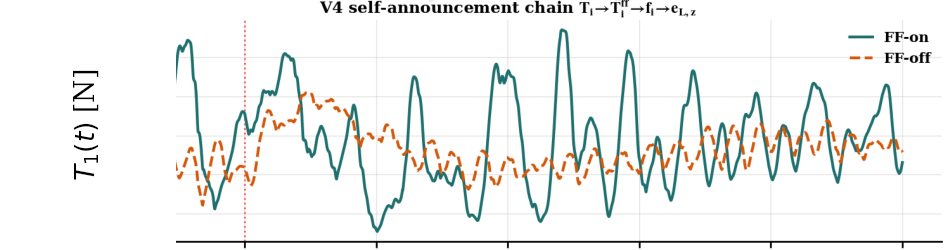
\includegraphics[width=\columnwidth]{Figures/fig_self_announcement_V4_a.png}%
    \label{fig:self-announcement-a}}\\[-0.5ex]
  \subfloat[Feed-forward command $T_1^{\mathrm{ff}}(t)$.]{%
    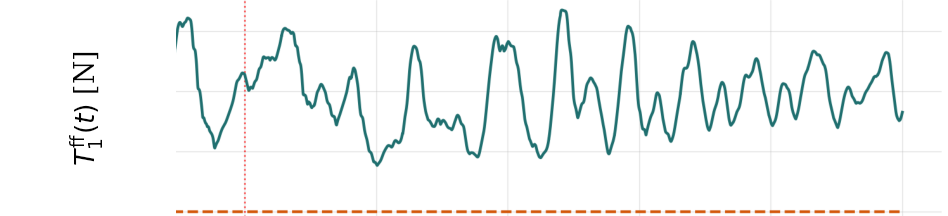
\includegraphics[width=\columnwidth]{Figures/fig_self_announcement_V4_b.png}%
    \label{fig:self-announcement-b}}\\[-0.5ex]
  \subfloat[Commanded thrust $f_1(t)$.]{%
    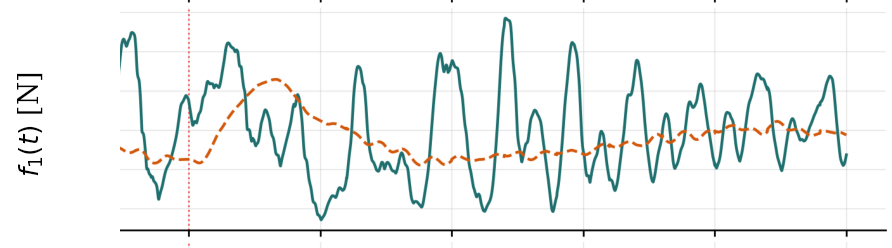
\includegraphics[width=\columnwidth]{Figures/fig_self_announcement_V4_c.png}%
    \label{fig:self-announcement-c}}\\[-0.5ex]
  \subfloat[Payload altitude error $e_{L,z}(t)$.]{%
    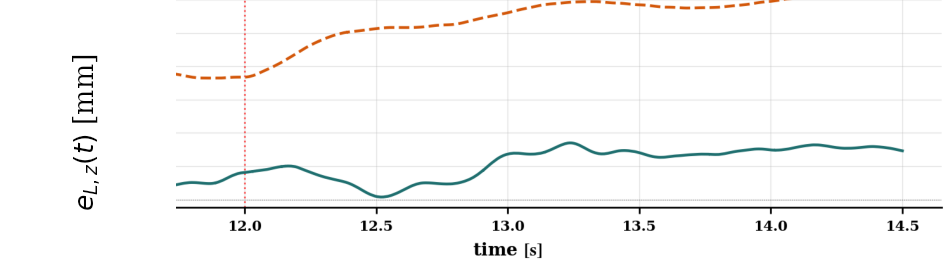
\includegraphics[width=\columnwidth]{Figures/fig_self_announcement_V4_d.png}%
    \label{fig:self-announcement-d}}
  \caption{Self-announcement causal chain (V4, fault~1, drone~0 severed at $t=\SI{12}{\second}$). Teal solid: baseline (FF-on); orange dashed: P2-A ablation (FF-off). With the identity active, $T_1^{\mathrm{ff}}$ tracks $T_1$ at the next tick (b), thrust steps proportionally (c), and altitude error stays bounded (d); with it disabled, $T_1^{\mathrm{ff}}\!=\!0$ flat, the thrust step is absent, and altitude error grows by $\sim\!\SI{300}{\milli\metre}$.}
  \label{fig:self-announcement}
\end{figure}

% ----------------------------------------------------------------
\subsection{Dwell-Time Boundary Characterisation}
\label{sec:VI-dwell}
% ----------------------------------------------------------------

\eqref{eq:dwell-assumption} asserts $\rho = e^{-\alpha_{\min}\tau_{\mathrm{pend}}} < 1$ for any $\tau_d > \tau_{\mathrm{pend}}$. V4 and V5 confirm two operating points inside the guaranteed regime but do not characterize behavior as $\tau_d$ approaches or falls below $\tau_{\mathrm{pend}}$. We close this gap with a boundary sweep on V4 across $\tau_d/\tau_{\mathrm{pend}} \in \{0.5, 0.75, 1.0, 1.25, 1.5, 2.0\}$ at seed~42.

For each point we compute the per-fault peak altitude excursion $\hat e_{p,z}^{\max}(t_k)$ relative to a 0.2-second DC-offset window ending at $t_k$ (removing the post-fault equilibrium shift), then form $\hat\rho(\tau_d) = \hat e_{p,z}^{\max}(t_2)/\hat e_{p,z}^{\max}(t_1)$. \Cref{fig:dwell-sweep} reports the result.

The empirical result is stronger than the hypothesis demands: $\hat\rho < 1$ at every tested dwell, including the sub-threshold $\tau_d=0.5\tau_{\mathrm{pend}}$ where $\hat\rho\approx 0.63$. The ratio falls to $\hat\rho\approx 0.14$ at $\tau_d=1.5\tau_{\mathrm{pend}}$. The non-monotonicity at $\tau_d=2.0\tau_{\mathrm{pend}}$ reflects the trajectory phase the second fault hits (centripetal peak vs trough); a fault-phase sweep would resolve it. The fault-2 peak is consistently below fault-1 across the sweep: the identity bounds the Lyapunov jump at each fault event (\cref{lem:jump-continuity}), and the inter-event contraction at rate $\alpha_{xy}$ (\cref{lem:horizontal-iss})---inducing the norm-level recovery rate $\lambda = \alpha_{xy}/2 = \SI{1.19}{\second^{-1}}$ of \cref{thm:hybrid-stability}---is sufficient to dissipate that bounded jump within each dwell interval, including the sub-threshold cases. H2 remains a structurally motivated bound; the empirical map shows contraction margin persists below it on this trajectory family.

\begin{figure}[htbp]
  \centering
  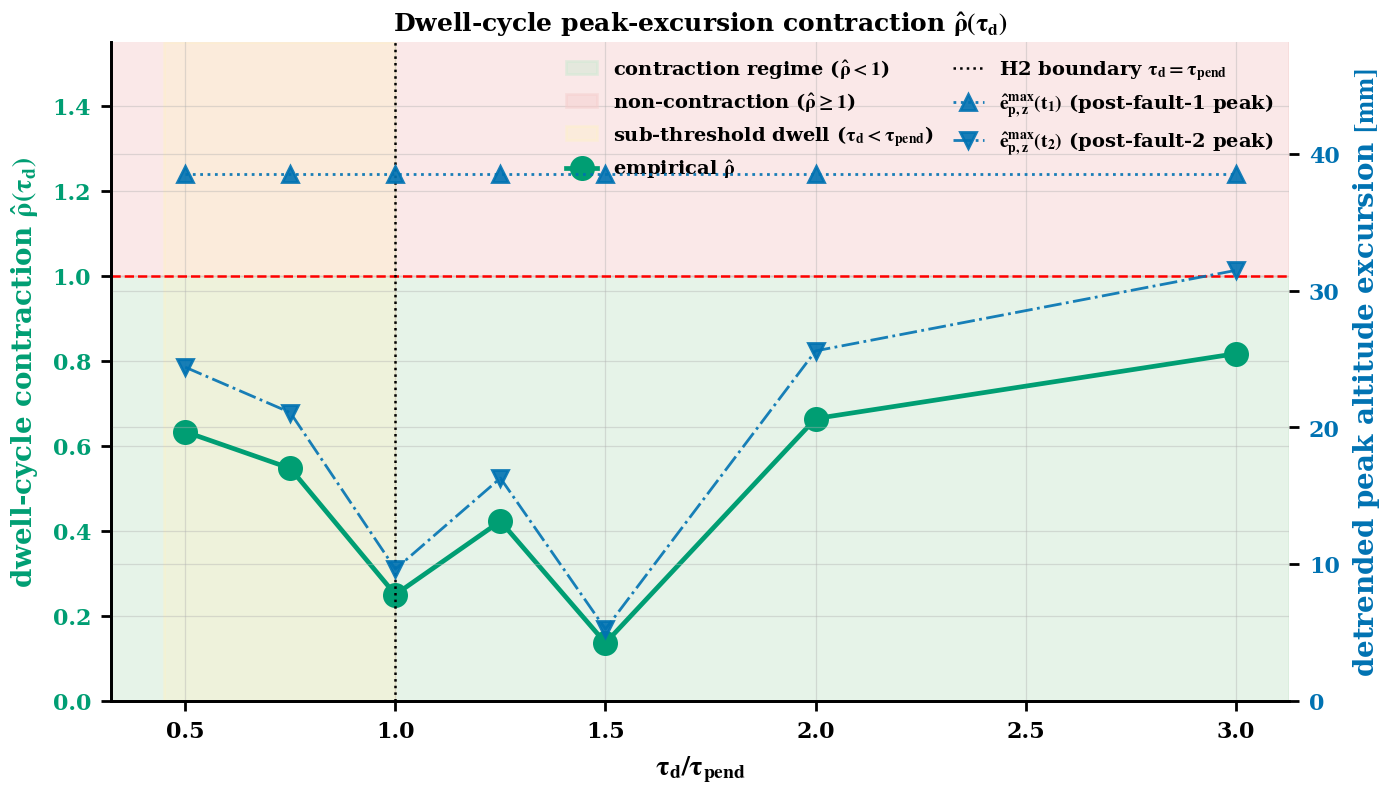
\includegraphics[width=\columnwidth]{Figures/fig_dwell_sweep.png}
  \caption{Dwell-cycle peak-excursion contraction $\hat\rho(\tau_d)$ versus normalised dwell $\tau_d/\tau_{\mathrm{pend}}$, V4 schedule, seed~42. Horizontal dashed: $\hat\rho=1$; vertical dotted: H2 boundary. $\hat\rho$ remains below unity across the full sweep, including sub-threshold dwell.}
  \label{fig:dwell-sweep}
\end{figure}

\subsection{Parameter Mismatch and Adaptive Augmentation}
\label{sec:VI-E}

P2-B evaluates robustness to payload-mass mismatch and the $L_1$ benefit (\cref{sec:l1-augmentation}, C3-$L_1$). We sweep $m_L \in \{2.5, 3.0, 3.5, 3.9\}~\si{\kilo\gram}$ (the PD design range, distinct from the $\SI{10}{\kilo\gram}$ V1--V6 payload) with $q^\star$ fixed at $\SI{3.0}{\kilo\gram}$ and compare FF-on, FF-off, FF-off$+L_1$. All runs use the fault-free trajectory to isolate mismatch effects. The $L_1$ evidence is obtained in rescue mode (FF off, $L_1$ alone), which isolates the $L_1$ contribution; main-mode evaluation at the canonical \SI{10}{\kilo\gram} point is follow-up work.

FF-on is robust across the range: RMSE varies $<1.9\%$, confirming the identity pre-compensates the per-drone load change without explicit mass estimation (\cref{cor:robustness}(i)). FF-off degrades approximately linearly, reaching $\SI{0.350}{\metre}$ RMSE at $m_L = \SI{3.9}{\kilo\gram}$ vs $\SI{0.341}{\metre}$ at the nominal. FF-off$+L_1$ recovers $\sim 40\%$ of the mismatch-induced sag.

The single-axis sweep of \cref{fig:l1-mass-mismatch} is one projection of the four-axis claim of \cref{cor:robustness}. The full response surface over $(m_L, k_s, c_{\mathrm{drag}}, \bar{w})$ on $n=100$ CRN-paired seeds is identified as a campaign extension.

\begin{figure}[htbp]
  \centering
  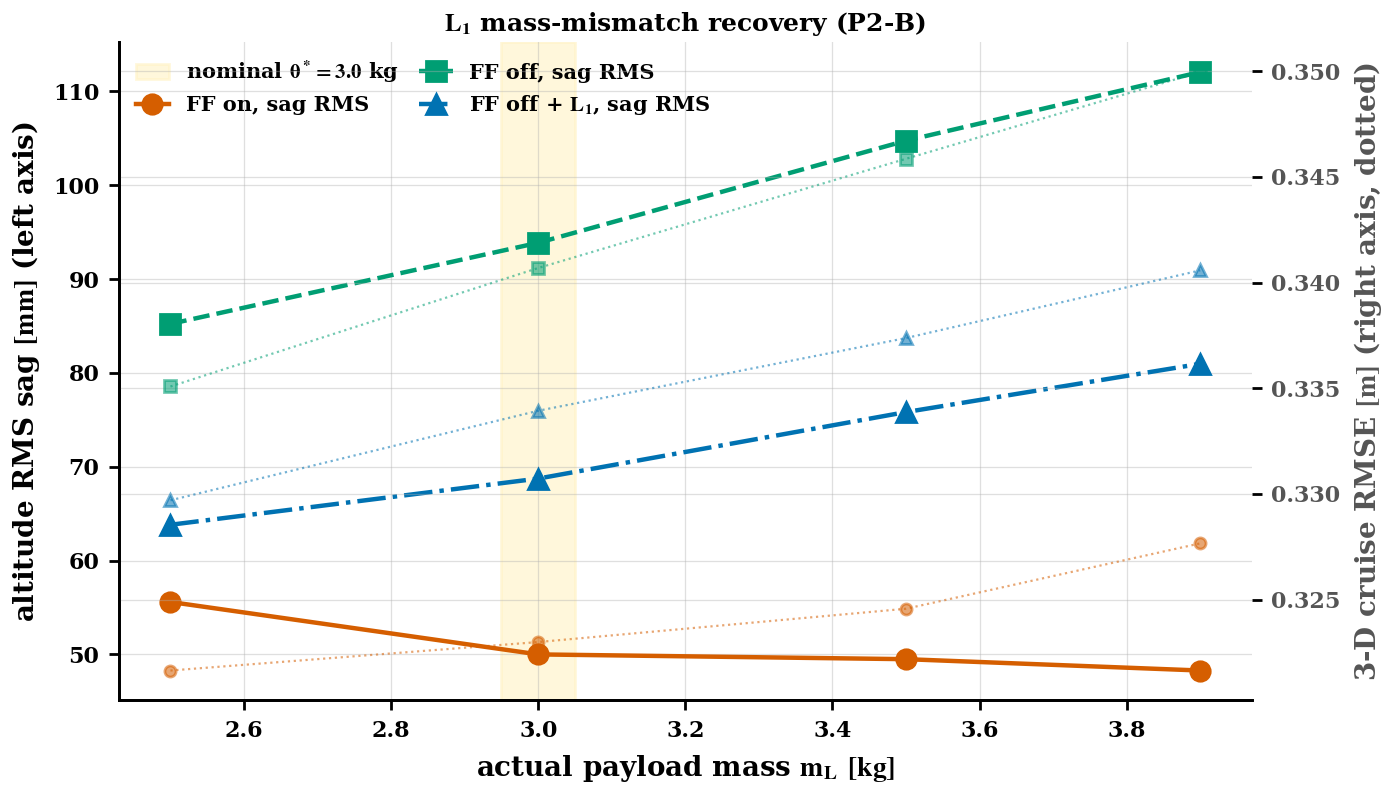
\includegraphics[width=\columnwidth]{Figures/fig_l1_mass_mismatch.png}
  \caption{P2-B payload-mass-mismatch sweep. Cruise-window 3-D RMSE versus $m_L \in \{2.5,3.0,3.5,3.9\}~\si{\kilo\gram}$ with $q^\star = \SI{3.0}{\kilo\gram}$ for FF-on, FF-off, and FF-off$+L_1$. FF-off$+L_1$ recovers $\sim 40\,\%$ of the FF-off-minus-FF-on sag gap.}
  \label{fig:l1-mass-mismatch}
\end{figure}

\paragraph{$L_1$ adaptive-gain stability map.} \Cref{prop:gamma-star} gives the scalar-proxy admissible window $\Gamma_{\min} \approx 1{,}190 < \Gamma < \Gamma^\star \approx 4.75\times10^5$. We sweep $\Gamma \in \{0.5, 2, 10, 30, 50, 80\} \times 10^3$ on a fault-free $\SI{20}{\second}$ mass-mismatch run ($m_L=\SI{3.9}{\kilo\gram}$ vs $q^\star=\SI{3.0}{\kilo\gram}$, FF off). Each drone runs its own $L_1$ update with the swept $\Gamma$, with no shared state or orchestrator. Altitude RMSE (\cref{fig:l1-stability-dashboard}) is highest at $\Gamma=500 < \Gamma_{\min}$ ($\SI{101}{\milli\metre}$, bandwidth-coverage insufficient), drops to a minimum of $\SI{88.5}{\milli\metre}$ at $\Gamma \approx 10^4$ (well inside the window), then rises mildly to $\SI{91.4}{\milli\metre}$ at $\Gamma=8\times 10^4$ (unmodelled cross-coupling). Peak sag follows the same shape, $\SI{130}{\milli\metre}$ down to $\sim\SI{113}{\milli\metre}$. The late-vs-early variance ratio stays in $[0.36, 0.37]$; no instability is observed across all six swept values ($\max_\Gamma\Gamma/\Gamma^\star \approx 0.17$). The unimodal shape, with the worst performance at the below-$\Gamma_{\min}$ point and the best within the window, empirically validates both bounds of \cref{prop:gamma-star}. Probing past $\Gamma^\star$ is follow-up work.

\begin{figure}[htbp]
  \centering
  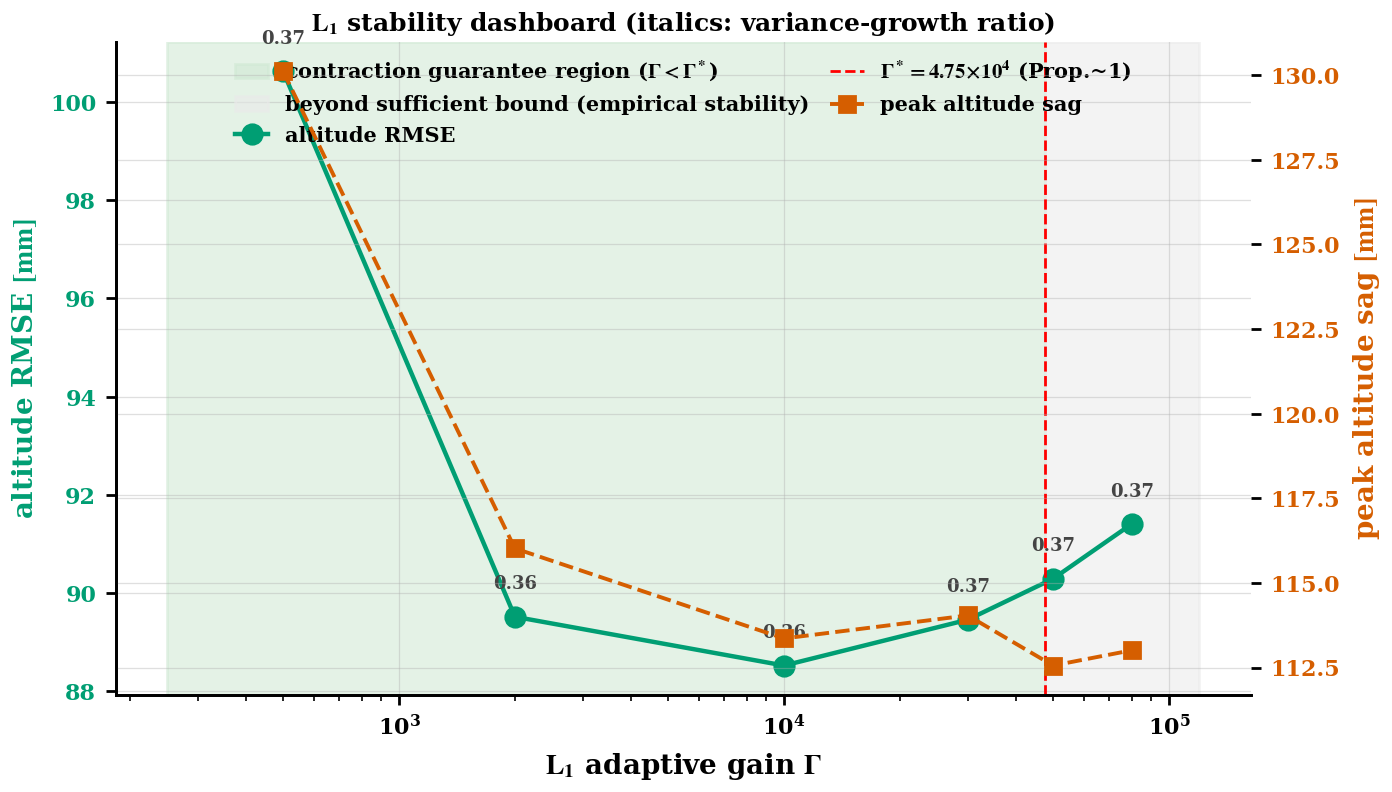
\includegraphics[width=0.92\linewidth]{Figures/fig_l1_stability_dashboard.png}
  \caption{$L_1$ adaptive-gain stability dashboard. Left axis (circles): altitude RMSE vs $\Gamma$. Right axis (squares, dashed): peak altitude sag. Italics: late-vs-early error-standard-deviation ratio. Green band: admissible window $\Gamma_{\min} \approx 1{,}190$ to $\Gamma^\star \approx 4.75\!\times\!10^5$ (\cref{prop:gamma-star}); the $\Gamma=500$ point lies below $\Gamma_{\min}$ and shows the highest RMSE, consistent with insufficient bandwidth coverage. FF-off rescue mode, $m_L=\SI{3.9}{\kilo\gram}$, no faults.}
  \label{fig:l1-stability-dashboard}
\end{figure}

% ----------------------------------------------------------------
\subsection{Extension Characterization and Binding-Regime
  Evidence}
\label{sec:VI-H}
\label{sec:VI-F}
% ----------------------------------------------------------------

P2-C and P2-D probe the MPC tension-ceiling (C3-MPC) and reshape supervisor (C3-Reshape) on V4. Both yield null findings on the canonical family, complemented by binding-regime probes for the operating conditions under which each extension activates.

\paragraph{P2-C --- MPC tension ceiling.} We sweep $T_{\max} \in \{60, 70, 80, 90, 100\}~\si{\newton}$ against the unconstrained baseline (\cref{tab:mpc-ceiling-sweep}).

\begin{remark}[NF2: MPC ceiling non-binding in canonical regime]
\label{rem:mpc-null}
  Peak tension during the fault transient is dominated by the pre-fault dynamic spike from the lemniscate's centripetal acceleration ($\approx \SI{42}{\newton}$ on survivors immediately before the first fault, resolving within one pendulum period); this spike is independent of the ceiling. The ceiling targets the post-fault quasi-static regime: at the 5$\to$3 transition with $\SI{10}{\kilo\gram}$ payload, $m_L g / 3 \approx \SI{32.7}{\newton}$, well below all tested ceilings. Lowering the ceiling from $\SI{100}{\newton}$ to $\SI{60}{\newton}$ produces no measurable change (NF2). The ceiling becomes binding when the post-fault load approaches $T_{\max}$---heavier payload, lower ceiling, or fewer survivors. \Cref{prop:mpc-slack,sec:theorem-preservation} preserve \cref{thm:hybrid-stability} whether or not the ceiling is binding.
\end{remark}

\paragraph{P2-D --- Formation reshape.} We sweep $T_{\mathrm{ref}} \in \{8, 10, 12\}~\si{\second}$ with and without reshape on V4, plus the aggressive-period binding-regime probe at $T_{\mathrm{ref}}=\SI{6}{\second}$ (E8). Peak post-fault rope tension is identical with reshape on and off at every tested period: $\SI{330.2}{\newton}$, $\SI{191.4}{\newton}$, $\SI{153.8}{\newton}$, $\SI{87.9}{\newton}$ at $T_{\mathrm{ref}} = 6, 8, 10, 12~\si{\second}$ respectively.

\begin{remark}[NF3: Reshape benefit zero across periods and aggressive-period probe]
\label{rem:reshape-null}
  The reshape supervisor targets the quasi-static-hover tension distribution under the symmetric-load-sharing model of \cref{thm:reshape}. At the tested periods, centripetal acceleration $a_c = (2\pi/T_{\mathrm{ref}})^2 A \approx 0.82$--$3.29~\si{\metre\per\second\squared}$ continuously modulates the per-rope distribution, and this dynamic modulation dominates the hover-equilibrium asymmetry the supervisor targets---so high centripetal load, far from making the asymmetry binding, makes it \emph{non}-binding. The quasi-static assumption of \cref{thm:reshape} therefore fails to bind at any tested period, including the aggressive $T_{\mathrm{ref}}=\SI{6}{\second}$ probe (E8) for which the linearised theorem a priori predicted a $\sim 25.8\%$ reduction; the measured benefit there is $0.0\%$. Pushing reshape into a binding regime would require a lower-bandwidth reference family or an extended objective accounting for the dynamic load. \Cref{thm:reshape,sec:theorem-preservation} preserve the envelope outside the binding regime.
\end{remark}

\begin{table}[htbp]
  \caption{MPC tension-ceiling sweep (P2-C, NF2). Peak rope tension and fraction of mission time over the commanded ceiling $T_{\max}$, V4 fault schedule.}
  \label{tab:mpc-ceiling-sweep}
  \centering
  \small
  \renewcommand{\arraystretch}{1.05}
  \begin{tabular}{crrr}
    \toprule
    Ceiling $T_{\max}$ & Peak $T$ & Peak post-fault & Time over ceiling \\
    \midrule
    60N       & 104.6N & 87.9N & 17.52\% \\
    70N       & 104.6N & 87.9N & 6.50\%  \\
    80N       & 104.6N & 87.9N & 1.60\%  \\
    90N       & 104.6N & 87.9N & 0.34\%  \\
    100N      & 104.6N & 87.9N & 0.12\%  \\
    Baseline & 104.6N & 87.9N & ---   \\
    \bottomrule
  \end{tabular}
\end{table}

% ----------------------------------------------------------------
\subsection{Trajectory-Phase Sensitivity of Recovery}
\label{sec:VI-fault-time}
% ----------------------------------------------------------------

V4 fixes $t_1=12$~s. We ask whether the recovery envelope depends on \emph{where in the lemniscate cycle} the first fault hits, i.e.\ whether $t_1{=}12$~s is fortuitous or representative. We sweep $t_1 \in \{8, 10, 12, 14, 16\}$~s on V4 with $\Delta t = 5$~s and the same fault drones, so the first fault lands at five distinct phases.

\Cref{fig:fault-time-sweep} shows peak post-fault sag and 3-D cruise RMSE. Peak sag varies from $\SI{12.0}{\milli\metre}$ ($t_1=14$~s, low-acceleration phase) to $\SI{55.4}{\milli\metre}$ ($t_1=12$~s, near a centripetal peak), a $4.6\times$ ratio exceeding the $3.6$--$4.0\times$ FF-ablation magnitude. 3-D cruise RMSE varies modestly, $\SI{313}{\milli\metre}$--$\SI{336}{\milli\metre}$ ($\sim 7\%$ range): cruise-window tracking is robust to fault phase even when per-event peaks are not. Canonical $t_1=12$~s sits at the upper end of the sag distribution---a worst-case phase, not a fortuitous one---which strengthens rather than weakens the recovery claims.

\begin{figure}[htbp]
  \centering
  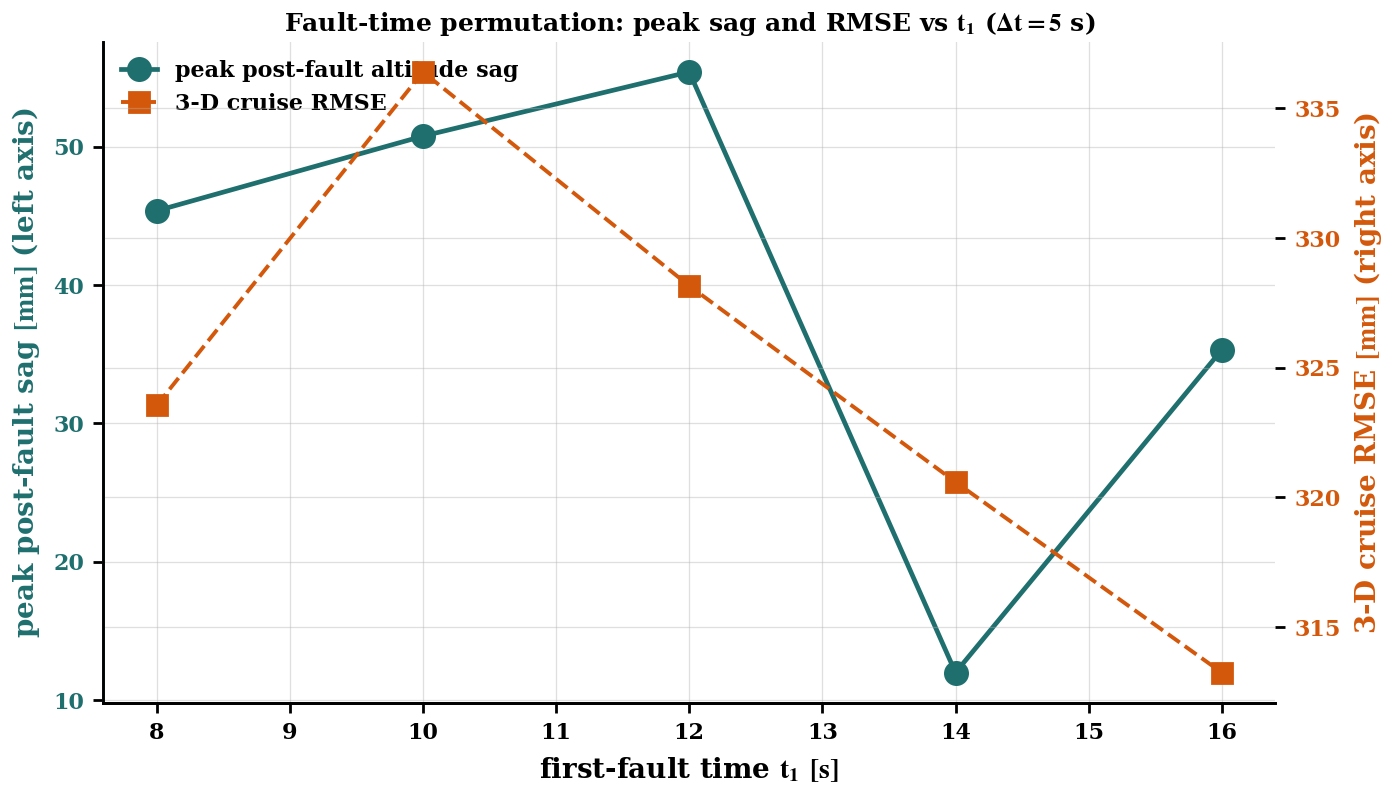
\includegraphics[width=\columnwidth]{Figures/fig_fault_time_sweep.png}
  \caption{Fault-time permutation. V4 dual-fault, $\Delta t=\SI{5}{\second}$, drones 0, 2; $t_1\in\{8,10,12,14,16\}$~s. Left axis: peak post-fault altitude sag. Right axis (dashed): 3-D cruise RMSE. The canonical $t_1=12$~s is a worst-case within the sweep.}
  \label{fig:fault-time-sweep}
\end{figure}

% ----------------------------------------------------------------
\subsection{H2 Sub-Threshold Dwell Probe}
\label{sec:VI-failure}
% ----------------------------------------------------------------

\Cref{fig:failure-gallery} shows the H2 violation probe: the sub-threshold dwell $\tau_d = 0.5\,\tau_{\mathrm{pend}} = \SI{1.12}{\second}$ on V4, with the Lyapunov proxy overlaid against the canonical V4 run. The sub-threshold trajectory is bounded and $\hat\rho$ (\cref{sec:VI-dwell,fig:dwell-sweep}) is below unity even here, showing the identity delivers contraction margin beyond H2's sufficiency. The probe illustrates the \emph{absence} of an empirical H2 failure on this family; constructing a regime that empirically violates contraction is follow-up work.

\begin{figure}[htbp]
  \centering
  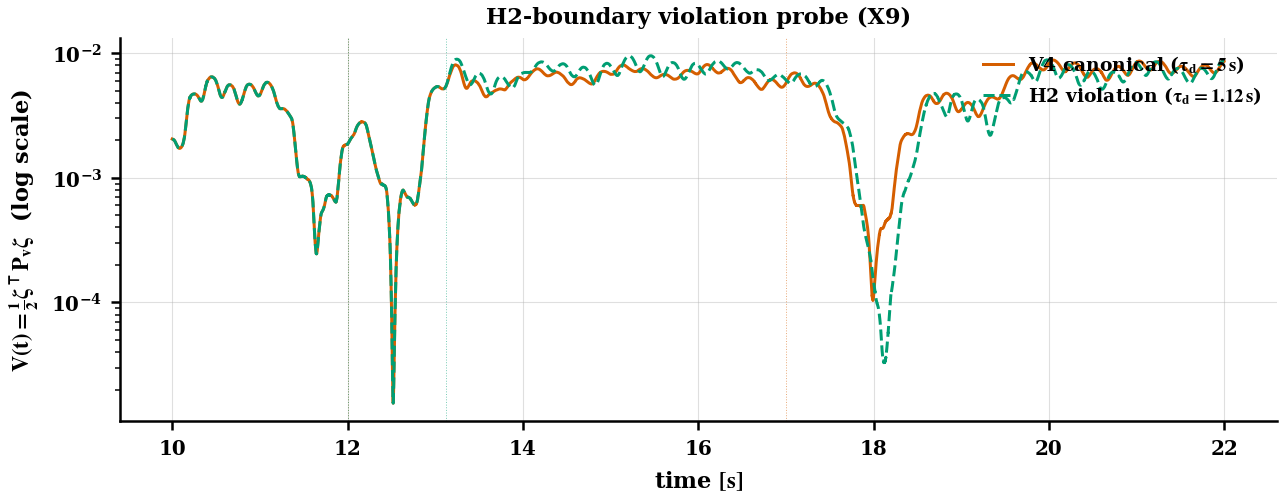
\includegraphics[width=\columnwidth]{Figures/fig_h2_violation.png}
  \caption{%
    H2 sub-threshold dwell probe. Lyapunov proxy $V(t)=\xi^\top P_v\xi$ at $\tau_d = 0.5\,\tau_{\mathrm{pend}} = \SI{1.12}{\second}$ overlaid with the canonical V4 trajectory ($\tau_d = 5\,\tau_{\mathrm{pend}}$). Red ticks: fault events. The sub-threshold trajectory remains bounded; $\hat\rho$ on the detrended peak-excursion definition of \cref{sec:VI-dwell} sits below unity (\cref{fig:dwell-sweep}).%
  }
  \label{fig:failure-gallery}
\end{figure}


\subsection{Actuator-Margin and Recovery-Time Audit}
\label{sec:VI-actuator-recovery}

A reviewer concern with cascade architectures is that the controller may rely on actuator saturation to absorb post-fault loads. We audit this with the per-drone maximum commanded thrust ratio $f_i(t)/f_{\max}$ over $[8,30]\,\si{\second}$ for V3--V6. The variant maxima are $0.73$ on V3, V4, V5 and $0.79$ on V6, all attained on drone~4, with zero cruise-window time above $0.9\,f_{\max}$ on every variant. The V3--V5 maxima coincide because the three variants share the first-fault schedule (drone 0 severs at $t=\SI{12}{\second}$) and the simulations are deterministic on a common wind seed: the variant peak is drone 4's transient at $t=\SI{12.68}{\second}$, $\SI{0.68}{\second}$ into the fault-1 recovery, and the second-fault spike (V4: $t=\SI{17}{\second}$, V5: $t=\SI{22}{\second}$) lands on a different drone with the trajectory at a different phase and stays below the fault-1 peak on drone 4. V6 reaches $0.79$ because the full-stack extensions ($L_1$ + MPC + reshape) shift the altitude command. Recovery is not actuator-limited on any variant.

\paragraph{Spike-then-relax thrust dynamics on V4.} The variant-level maximum hides the intra-fault dynamic that directly evidences H2 on the actuator channel. \Cref{tab:thrust-transient} reports, per V4 survivor ($i\in\{1,3,4\}$), the within-1\,s peak commanded thrust at each fault and the settled mean 2--4\,s after. Survivors show a $1.18$--$1.79\times$ peak-over-settled overshoot, decaying to a new steady state within $\sim \tau_{\mathrm{pend}}\approx\SI{2.24}{\second}$. Steady-state thrust per survivor rises $+25$ to $+34\%$ vs the pre-fault baseline; the survivor sum settles near $\SI{179}{\newton}$ at $t \in [27,30]$\,s, balancing $m_L g + 3 m_{\mathrm{drone}} g \approx \SI{142}{\newton}$ plus centripetal/tilt overhead---an independent check of the post-fault load redistribution. This is the actuator-channel signature of the same recovery the Lyapunov-proxy contraction of \cref{sec:VI-C} reports for the state error.

\begin{table}[htbp]
  \caption{V4 spike-then-relax thrust dynamics on the three surviving drones. Peak: max within 1\,s of each fault; Settled: mean 2--4\,s after the fault. $\Delta$: steady-state increase ($t\!\in\![27,30]$\,s) over the pre-fault $[10,12]$\,s baseline.}
  \label{tab:thrust-transient}
  \centering
  \small
  \begin{tabular}{cccccc}
    \toprule
    Drone & Fault & Pre & Peak & Settled &
      Peak/Sett. \\
    & & (N) & (N) & (N) & ratio \\
    \midrule
    1 & f1 ($t_1{=}12$ s) & 59.3 &  82.2 & 62.1 & $1.32\times$ \\
    1 & f2 ($t_2{=}17$ s) & 62.1 &  97.2 & 69.1 & $1.41\times$ \\
    3 & f1                 & 40.7 &  53.4 & 40.1 & $1.33\times$ \\
    3 & f2                 & 40.1 &  77.8 & 52.2 & $1.49\times$ \\
    4 & f1                 & 41.7 & 110.0 & 61.4 & $1.79\times$ \\
    4 & f2                 & 61.4 &  63.3 & 53.7 & $1.18\times$ \\
    \midrule
    \multicolumn{6}{l}{\emph{Steady-state ($t\in[27,30]$\,s) vs pre-fault baseline:}} \\
    1 & --- & 53.3 & --- & 75.1 & $\Delta = +34\,\%$ \\
    3 & --- & 42.8 & --- & 53.0 & $\Delta = +25\,\%$ \\
    4 & --- & 42.4 & --- & 50.8 & $\Delta = +26\,\%$ \\
    \bottomrule
  \end{tabular}
\end{table}

\Cref{tab:recovery-iae} reports per-fault metrics beyond cruise RMSE: peak error norm, peak sag, recovery time $t_{\mathrm{rec}}$ to within $\varepsilon = \SI{0.35}{\metre}$ for $\SI{0.3}{\second}$ continuous, and IAE over $\tau_{\mathrm{pend}}$ post-fault. $t_{\mathrm{rec}}$ is bounded by the next fault's arrival in dual-fault variants; IAE captures the integrated per-event cost.

\begin{table}[htbp]
  \caption{Per-fault recovery metrics. $t_{\mathrm{rec}}$ threshold $\SI{0.35}{\metre}$ (3-D, $\SI{0.3}{\second}$ continuous hold); IAE integrated over $\tau_{\mathrm{pend}}$ or the gap to the next fault, whichever is shorter.}
  \label{tab:recovery-iae}
  \centering
  \small
  \begin{tabular}{llccccc}
    \toprule
    Variant & Fault & $t^\star$ & peak $\|e\|$ &
      peak sag & $t_{\mathrm{rec}}$ & IAE \\
    \midrule
    V3 & 1 & 12.0s & 481mm & 85mm & 0.00s & 0.52m$\cdot$s \\
    V4 & 1 & 12.0s & 481mm & 85mm & 0.00s & 0.52m$\cdot$s \\
    V4 & 2 & 17.0s & 457mm & 89mm & 0.32s & 0.70m$\cdot$s \\
    V5 & 1 & 12.0s & 481mm & 85mm & 0.00s & 0.52m$\cdot$s \\
    V5 & 2 & 22.0s & 469mm & 90mm & 1.58s & 0.81m$\cdot$s \\
    V6 & 1 & 12.0s & 481mm & 73mm & 0.00s & 0.51m$\cdot$s \\
    V6 & 2 & 17.0s & 460mm & 72mm & 0.33s & 0.70m$\cdot$s \\
    \bottomrule
  \end{tabular}
\end{table}

% ----------------------------------------------------------------
\subsection{Reproducibility and Claim-to-Evidence Map}
\label{sec:VI-G}
\label{sec:reproducibility}
% ----------------------------------------------------------------

\begin{remark}[Simulation protocol and seed manifest]
\label{rem:reproducibility}
  V1--V6 use fixed Dryden seed~42, producing bit-exact output across runs at identical Drake and library versions. Inter-variant RMSE differences are therefore attributable to controller configuration and fault schedule on this common realization. The principal ($+x$) wind component achieves a $2\sigma$ exceedance within $[8,12]$~s, making this a reproducible stress case.

  Ablations (P2-A through robustness sweep) are deterministic point estimates at seed~42; CRN-paired replication yielding bootstrap CIs is follow-up work. The seed manifest and all simulation artifacts are publicly available in the companion repository~\cite{tether_grace_code}.

  \textbf{Scope of H1--H3 certification.} \Cref{tab:domain-audit} certifies domain membership for the demonstrated mission family only. For a new trajectory, reference profile, wind envelope, or fault schedule, the same gate audit must be repeated before invoking the conditional certificate.
\end{remark}

The audit trail: C1 is supported by \cref{tab:domain-audit,tab:reduction-residuals}; C2 by \cref{fig:fault-zoom,fig:dwell-sweep}; C3 by \cref{fig:l1-stability-dashboard}; FF causality by \cref{tab:ff-ablation,fig:self-announcement}; actuator margin and recovery time by \cref{tab:thrust-transient,tab:recovery-iae} (with the variant-level maxima reported inline in \cref{sec:VI-actuator-recovery}); operating-boundary characterisation by \cref{sec:VI-failure}.
